\documentclass{article}
\usepackage[utf8]{inputenc}

\title{Final Exam }
\author{wbg231 }
\date{November 2022}
\usepackage{tikz,graphicx,hyperref,amsmath,amsfonts,amscd,amssymb,bm,cite,epsfig,epsf,url}
\begin{document}
\begin{itemize}
\maketitle
%\section{question number}
%\subsection{problem statement}
\section{Question 1}

%\item 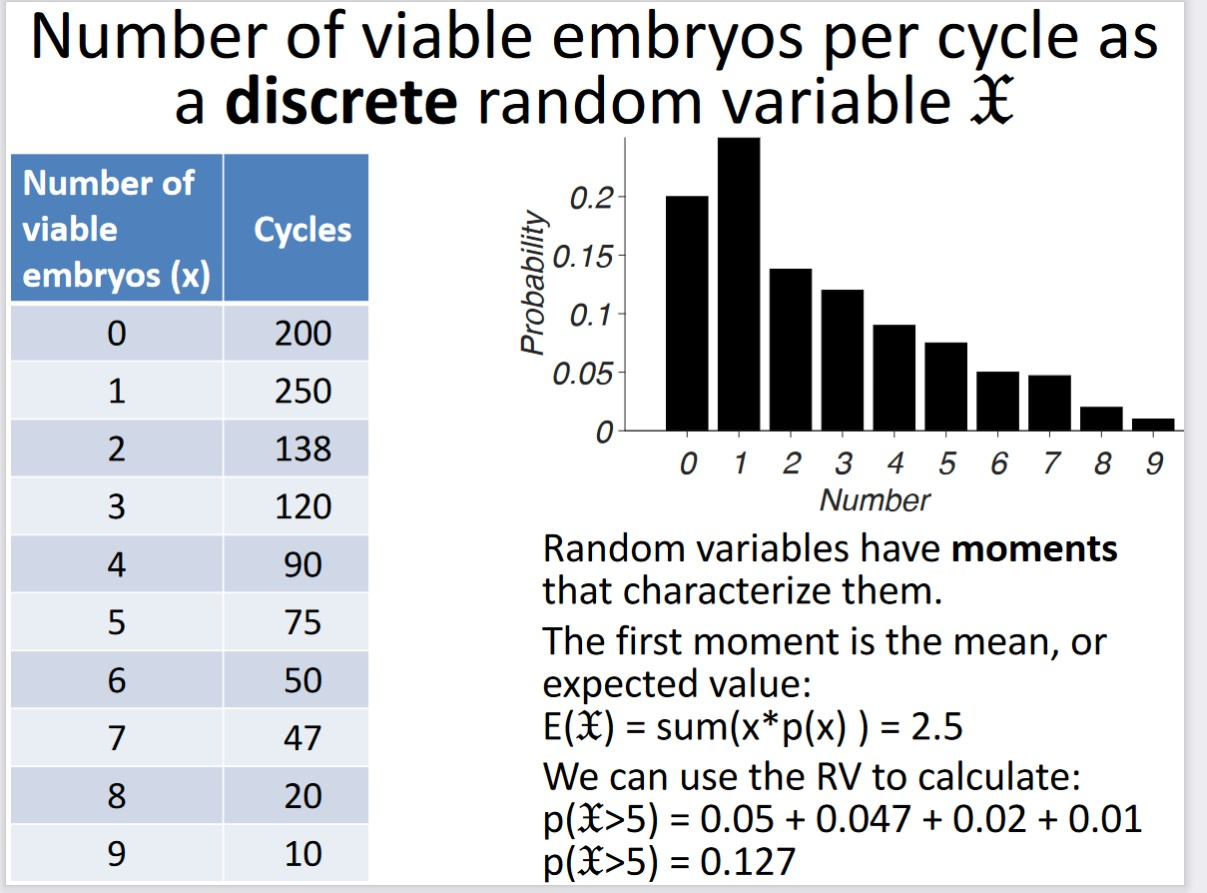
\includegraphics[width=7.5cm]{Final_Review/Lecture_2/lecture_1example.jpg}
\subsection{problem statement}
\item you have three groups you want to compare against each other. You decide to run multiple t-tests (3 in total) and use a Benferroni correction for $\alpha=.05$ what is your alpha after the correction?

\subsection{working}
\item what is a Benferroni correction? 
\item here is a yt video on it https://www.youtube.com/watch?v=HLzS5wPqWR0
\item from lab 3" We can do as many t-tests as we want. We will have to adjust the alpha-level from 0.05 to 0.05/c, where c is the number of tests (comparisons), that's called the "Bonferroni correction"."
\item we are doing 3 tests so $\alpha_{adjusted}=\frac{.05}{3}=\frac{1}{60}$

\section{question 2}
\subsection{problem statement}
\item you are studying the relationship between smoking and heart health. you find that there is a correlation of $r=-.84$. while notifying your team of your findings, your colleague says .
what about their family history of heart disease?" what is your next step?
\subsection{initial thought}
\item multiple regression to control for this 
\subsection{process of elimination}
\item option one is likely wrong because it is about the relationship between smoking and family history 
\item option 3 is like wrong because it is about the relationship between family history and health 
\item so it should be option 2

\section{question 3}
\subsection{problem statement}
\item what does this symbol mean $\Sigma\Sigma$?
\subsection{working}
\item email pascal if this is literally meant to just be two sigmas 
\item if so, it would have to be evaluated as $\Sigma\Sigma$


\section{question 4}
\subsection{problem statement}
\item $15\%$ of all students are in the human ties, 58\% of students are undergraduates. 19\% of undergraduates are in the humanities. what is the likelihood that a random humanities student is an undergraduate
\subsection{working }
\item let $h$ be event a student is in the humanities $P(H=1)=.15$
\item let u be event a student is an undergraduate $P(u=1).58$
\item we are that 19\% of undergrads are in the humanties in other words $.19=\frac{P(U=1\cap H=1)}{P(u=1)}=P(h=1|u=1)$
\item we are trying to find $P(u=1|h=1)=\frac{P(u=1\cap h=1)}{p(h=1)}=\frac{P(h=1|u=1)P(u=1)}{P(h=1)}=\frac{(.19(.58)}{(.15)}=.735$


\section{Question 5}
\subsection{problem statement}
the variance of a column in this text file is 7, what is the standard error of the mean 
\subsection{working}
\item standard error of mean is $SEM=\frac{\sigma}{\sqrt{n}}=\frac{\sqrt{7}}{n}$


\section{question 6 }
\subsection{problem statement}
\item which of the following is true about confounding variables
\subsection{process of elimination}
\begin{enumerate}
    \item could be true 
    \item this is true 
    \item this is true 
    \item this is true 
    \item so it is all of the above
\end{enumerate}


\section{question 7}
\subsection{problem statement}
\item class is rescheduled because of a Holiday. the professor has a .7 chance of noticing before hand. there are 200 students each with a .01 chance of noticing it. who is more likely to notice first? the professor or the students? 
\subsection{working }
\item this is kind of a weird question
\item assume that they mean the chance of the prof noticing at each discrete time step is .7 that is 70\%
\item while the chance of each of the the 200 students noticing at each discrete time step is .01\% 
\item it does not say that the chance of each stunted noticing are independent but lets assume that is true 
\item lets also assume it is true at each time step
\item so we can view this as a geometric rv
\item the likelihood of the prof noticing at time t is $P(x=t)=(.7)(.3)^{t-1}$
\item the mean of this thing is $\frac{1}{.7}=1.5 time steps$
\item we model the students as independent so lets think of that as a product of 200 geometric rvs with pmf $P(s=t)=(.01)(.99)^t$ each 
\item so simulate 200 students at each time step and take the min 
\item then see which has a lower mean 
\item it ended up quantitatively being the students
\item ask Pascals about assumptions 
\section{question 8}
\subsection{problem statement}
\item the text of this one is confusing 
\subsection{working}
\item i think there are meant to be 3 categories so the degrees of freedom in the Chi squared is 3-1=2
\item alternatively if the words at the front indicate row categories and the others are col categories then degree's of freedom are (r-1)(c-1)=(2-1)(3-1)=2 so it still works i think 


\section{question 9}
\subsection{question text}
\item the main idea behind the PCA is to
\subsection{process of elimination}
\begin{enumerate}
    \item reduce the number of dimensions (true)
    \item separate explained variance from unexplained variance, PCA is about reducing the dimensionality of our predictors i don't think there is really a concept of explained or unexplained variance here
    \item eliminate outliers (false)
    \item test if one has enough power (false)

\end{enumerate}    
    
 \section{question 10}
 \subsection{text}
 \item in a linear regression with one independent variable (x), there are how many degrees of freedom? 
\subsection{working }
\itme at 13 minutes into zoom recording of lecture 10 they say degrees of freedom is the degree of your model. 
\item on lecture 4 slide 18 pascal says, "The number of independent pieces of information
(numbers, measurements, data points) in a dataset
that a parameter calculation is based on."
\item in linear regression we are estimating$\beta_0$ and  $\beta_1$, and we have the data $x_1...x_n$ so that would imply that we have n points to estimate 2 parameters and thus n-2 total degrees of freedom 
\item we are not given the number of n so not enough information is given 
\section{question 11 }
\subsection{problem statement}
\item the Mann-Whitney u test and Krystal-Wallis test are both based on?
\subsection{process of elimination}
\begin{enumerate}
    \item calculating the rank sum (this is true for Mann-Whitney u test i googled it and also seems to hold for the other so this is true) 
    \item dividing up the variance into variance explained and unexplained (false i don't think either have to do with variance explained or unexplained they are hypothesis tests)
    \itme comparing means (these are both non-parametric so clearly false)
    \item comparing distributions (the Mann-Whitney u test u compares the median not the distribution) 
\end{enumerate}

\section{question 12}
\subsection{problem statement}
\item how does increasing $\alpha$ effect the required sample size for a certain level of power? 
\subsection{process of ellimination}
\begin{enumerate}
    \item increase it ($\alpha$ is our chance of making a false positive, so if we make alpha higher we are more likely to have a false positive, but also thus less likely to have a false negative (so power goes up) thus to keep our power the same we need to lower sample size) 
    \item decreases it  (by option 1 logic this is true) 
    \item power does not affect same size (this is true but not related to the question) 
\end{enumerate}
\section{ question 13}
\subsection{question text}
\item Mad differs from the standard deviation in that 
\subsection{process of elimination}
\item mad is defined as $Median(\Sigma|x-median(x)|\frac{1}{n})$ standard deviation is $\sqrt{\Sigma\frac{(x-\Bar{x}}{n}}$
\begin{enumerate}
    \item it described the central tendency of a sample (false that is the goal of both)
    \item It us less robust to extreme values (false it is a median)
    \item it doesn't square now take the square root ( true in terms of the formula, also by not squaring things it is further robust to outliers so i think that is by design )
    \item it divides by the number of the sample (false)
    \item is more common (false)
    \item none of the above (depends on how we feel about c i think c is true)
\end{enumerate}
\section{question 14}
\subsection{problem text}
\item logistic regression is similar to a linear regression except:
\subsection{process of elimination}
\begin{enumerate}
    \item the log odds of the dependent variable is considered (the logistic takes x ie the independent as input uses some scalar beta to transform it and returns the log odd of y ie the dependent variable to this is true)
    \item the log odds of the independent variable is considered 
    \item the log probability of the dependent variable is considered (we look at the odds not the probability so false) 
    \item the log probability of independent variable is considered
    \itme the odds ratio of the dependent variable is consider d
    \item the odds ratio of the  independent variable is considered (we take the logs so false)
\end{enumerate}

\section{question 15}
\subsection{problem statement }
\item a researcher suspects that there is a confound call it z that mediates the correlation between x and y. the researcher runs a partial correlation between x and y while controlling for z. this correlation is obtained by: 
\subsection{process of elimination}
\item there is some math i am unfamiliar with here, look over the Wikipedia page, the linear algebra explanation seems to make sense that option c is correct. 
\begin{enumerate}
    \item correlating x with z (false tell us nothing about x and y)
    \item correlating y with z (false tells us nothing about x and y) 
    \item correlating the residuals from the regression between x and z with the residuals from the regression between y and z  (true according to wikipedia) 
    \item decomposing the variance of z. ( i am not sure what they mean by this) 
\end{enumerate}
\section{question 16}
\subsection{problem statement}
\item study is done.... they report $t(9)\=1.58, p\leq .05$ for correlated groups. you can conclude that 
\subsection{process of elimination}
\begin{enumerate}
    \item there were 9 models in the study (they say this was done using a t test for correlated groups it would make sense that the $t(9)$ they are referring to means they used a t distribution with 9 degrees of freedom. the correlated t test has n-1 degrees of freedom so if this interpretation was correct we would have 10 models false)
    \item they preformed a t-test for independent groups ( they say they did a t test for correlated groups 
    \item Cohen huge ( we have nothing about the means of sigma of the sample so we can not calculate this). 
    \item effect size big according to Cohen
    \item Cohen moderate
    \item none of the above (this has to be true)
\end{enumerate}
\section{question 17}
\subsection{question text}
\item In PCA the Kaiser Criterion indicates that factors with an eigenvalue of x or above should be kept what is x?
\subsection{solution}
\item it is 1. 
\item this was discussed in lab 11 at like 17 minutes
\item when we do pca we z score the eigenvalues, so that is we take for eigenvalue $\lambda_i$ we get $\lambda_{iz}=\frac{\lambda_i-\Bar{\lambda}}{\sigma_\lambda}$ so if $\frac{\lambda_i-\Bar{\lambda}}{\sigma_\lambda}\leq 1$ that means the eigenvalue is less than one standard deviation away from the mean and thus is not important. Also note given input matrix x we do pca on $X^TX$ ie the correlation matrix which is positive definite so all eigenvalues are positive
\section{question 18}
\subsection{question text}
\item in a chi squared distribution the probability distribution grows higher and moves to the left as the distribution narrows as the degrees of freedom do what?
\subsection{working}
\item look at about 1 hour and 34 minutes into lecture 4, as the degrees of freedom go down the distributing moves to the right and the standard deviation goes down 
\item so decrease is the answer
\section{question 19}
\subsection{problem text}
\item ask 4 people to rate 100 head shots on attractiveness your degrees of freedom are
\subsection{working / process of elimination }
\item degrees of freedom are The effective sample size that
a parameter calculation is based on (number of true
variables or independent data points)
\item we know that we have 4 people each rate 100 head shots and will use that to predict something so that is a total of 4(100)=400 data points
\item we have yet to do any comparison so there is no reason to think we have lost degrees of freedom so i would stick with 400
\item keep thinking about it, one of the last questions is super similar and does not even list the same number of samples as an option so that may be wrong, i am still confused exactly why that would be the case though.

\section{question 20}
\subsection{problem text}
\item you want to know if people who have a goatee are perceived as more attractive. you have 10 models. the most powerful design to reveal there is a difference is to

\subsection{working / process of elimination }
\begin{enumerate}
    \item randomly pick 5 models with a goatee and 5 models with out a goatee and ask people to rate them then do a t test for independent groups 
    \item pick 10 models with and with out a goatee rate them before and after shaving then do a t test for correlated groups (true this is the better test, as it controls for inter individual variability) 
    \item do a z test on 5 with goatee and five without goatee (false since we don't have population parameters we can not do this)
    \item do a z test 10 with goatee then have them shave it (false)
    \item this is a trick question 10 models is not enough to show anything (false, since does not answer the question) 
    \item none of the above 
\end{enumerate}
\section{question 21}
\subsection{problem text}
\item in a certain populating the likelihood of having 0 through 6 children is [8,8,12,23,18,15,16] in percents, what is the likelihoods that a random family has 4 or more kids
\subsection{working / process of elimination }
\item they say in the family there are a lot of families in the town 
\item and that this town has a unique distribution of number of kids
\item so we can treat it as a population
\item we can just think of that as a random variable with those values as pmf, then we can find the cdf.
\item we in other words the likelihood is just 18+15+16\%=.49 which is about 50 


\section{question 22}
\subsection{problem text}
want to see if students skip breakfast. you sample 100 students and ask if they skip breakfast. if you wanted to do a chi squared test for significance what would be the expected frequency for each category (breakfast vs does not have breakfast) 
\subsection{working / process of elimination }
\item we are studying if students skip breakfast 
\begin{enumerate}
    \item 50 in each category (i guess assuming our null that it is equally like this is true) 
    \item 25 in each category (false does not add up to 100)
    \item 30 in each category (false does not add up to 100)  
    \item there are not categories the expected frequency is 100 ( we need to divide by expected count in the formula so the expected count for no class can be 0) 
\end{enumerate}
\section{question 23}
\subsection{problem text}
\item the likelihood of getting stuck in a certain elevator is .4. so the odds of doing so are 
\subsection{working / process of elimination }
\item odds of an event a are $\frac{P(a)}{P(a^c)}$ so in this case that is $\frac{.4}{.6}$

\section{question 24}
\subsection{problem text}
the t distribution approximates this distribution  with a large n

\subsection{working / process of elimination }
\item the normal distribution, that is the whole point
\item lecture 4 slide 23 

\section{question 25}
\subsection{problem text}
\item that does simple linear regression minimize?
\subsection{working / process of elimination }
\begin{enumerate}
    \item the sum of the differences between predicted value and measurements (false)
    \item the sum of the squared differences between predicted values and measurements (true) 
    \itme sum of the absolute value... (false) 
    \item the sum of the cube (false)
    \item none of the above 
\end{enumerate}


\section{question 26}
\subsection{problem text}
\item which of the following events are mutually exclusive? 
\subsection{working / process of elimination }
\begin{enumerate}
    \item opening a package and discovering (a working product) or (a malfunctioning product)  ( true if we assume that malfunctioning and working are opposite states.)
    \item opening two packages and (the first one works ) but (the second one does not) (false you can have have both of these events happen) 
    \itme being 65 and retired (false this should be the case)
    \item being 7 and playing the piano (false) 
    \item color of a butterfly and the number of creator's on the moon (false these are completely unrelated) 
    \item none of the above (looks true) 
\end{enumerate}

\section{question 27}
\subsection{problem text}
\item in an independent samples t test one losses how many degrees of freedom by calculating the means? 
\subsection{working / process of elimination }
\item we calculate the mean of each sample and thus two means so 2. 


\section{question 28}
\subsection{problem text}
\item to detect a small effect size one will need X to get adequate power
\subsection{working / process of elimination }
\begin{enumerate}
    \item a small sample (this will further reduce power so false)
    \item about 100 participants (power depends on effect size so false in some cases)
    \item a large sample (true )
    \item a lot of confidence (this is unrelated) 
\end{enumerate}

\section{question 29}
\subsection{problem text}
\item you run a multiple regression to learn how much ethnicity predicts income, while controlling for education gender and age. conceptually this means which of the following?
\subsection{working / process of elimination }
\begin{enumerate}
    \item how much of the variance in income is predicted by ethnicity regardless of those other factors (I don't love the word regardless here, but if you take regardless to mean holding equal then i mean the beta on that variable is that, so this seems to be the least weird)
    \item how much of the variance in ethnicity is predicted by income regardless of education gender or age ( this has the the variables backwards so false )
    \item who has the highest income in each category (false) 
    \item the relationship between ethnicity and education (false this gives you the relationship controlling for these things but there could be other confounds) 
\end{enumerate}
\section{question 30}
\subsection{problem text}
\item when you decrease $\alpha$ level you increase 
\subsection{working / process of elimination }
\begin{enumerate}
    \item power (power goes down with $\alpha$ since you are overall more strict about what p-values you take
    \item the p value (this is related to the sample not alpha )
    \item type 1 error ( this is $\alpha$ so if $\alpga $ goes down this goes down 
    \item type 2 error (power is $1-\beta$) so if $1-\beta$ has gone down that means that $\beta$ which is our likely hood making a type II error has gone up so true) 
\end{enumerate}

\section{question 31}
\subsection{problem text}
\item how does the t distribution differ from the normal distribution at a small value of n 
\subsection{working / process of elimination }
\item a small value of n means low degrees of freedom 
\item the z has a lower peak, and fatter tails at lower degrees of free dome
\item it is not skewed though. 
\item so the pollution is A just fatter fails. 



\section{question 32}
\subsection{problem text}
\item the chi squared test is based on calculating the difference between: 
\subsection{working / process of elimination }
\begin{enumerate}
    \item observed and expected frequencies (true that is waht hte test does)
    \item sample means and population means (false: does not make sense for categorical data)
    \item explained and unexplained variance (false that is only a thing for predictors) 
    \item mean squares ,,, (false the mean does not make sense for categorical data) 
\end{enumerate}
\section{question 33}
\subsection{problem text}
\item the probability of two independent events happening is 
\subsection{working / process of elimination }
\item For two events A and B they are independent $  \iff P(a\cap b)=p(a)p(b)$ 
\item and $P(A\cap B)$ means that a and b happened so that is what we are looking for 
\item so it is the product 
\begin{enumerate}
    \item is the sum of the probabilities (false)
    \item is the product of the probabilities (true) 
    \item can be computed based on conditional probabilities (this is always true $P(a\cap b)=P(a|b)P(b)$ where if a and b are independent we have $P(a|b)=P(a)$  thus  $P(a\cap b)=P(a)P(b)$ so it is true, but not needed 
    \item can be computed based on Bayes rule ( we can use Bayes rule to compute this but Bayes is for inverting converting conditional probabilities, and it is unnecessary either way in this case)  
\end{enumerate}

\section{question 34}
\subsection{problem text}
\item one would think about running a Mann-Whitney u test instead of a t test when: 
\subsection{working / process of elimination }
\begin{enumerate}
    \item the data is not normally distributed ( true: the t test does assume that the data is distributed normally, it also assume the mean or what ever sample parameter we are looking for is meaningful. the  Mann-Whitney u test does not require the data is normally distributed so this is for sure a case where you would use it )  
    \item the data is less than interval scale level ( interval scale level just means that the distance between each unit of analysis is the same, like the integers are all spaced by 1. the Mann-Whitney u test does not require this so we can use it for ordinal data like ratings or satisfaction measures so this is also true. \href{https://www.questionpro.com/blog/nominal-ordinal-interval-ratio/}{here is an article on it }. )
    \item both 1 and 2 (so yeah both are true)
    \item there is no difference (false) 
\end{enumerate}

\section{question 35}
\subsection{problem text}
\item a person has two children and one is a son. what is the likelihood the other is a daughter
\subsection{working / process of elimination }
\item the only possible cases are (b,b),(b,g),(g,b),(b,b)
\item let $x_i$ represent the gender of kid i and it can take on a value of 1 if the kid is a daughter
\item we want $P((x_1=i,x_2=j)|(x_1=0\cup x_2=0))$ where $i\neq j$
\item so to break that down that is the even that the two kids have different gender given there is at least one son 
\item 
$P((x_1=i,x_2=j)|(x_1=0\cup x_2=0))=\frac{P((x_1=i,x_2=j)\cap(x_1=0\cup x_2=0))}{(x_1=0\cupx_2=0)}$ since at least one being a boy is a subset of them having different genders we can write $ =\frac{P((x_1=i,x_2=j)}{(x_1=0\cup x_2=0)}=\frac{\frac{2}{4}}{\frac{3}{4}}=\frac{2}{3}$ 
\section{question 36}
\subsection{problem text}
\item if the sampling is independent and represent (each member of the population has an equal chance of being in the sample mean) then X parameter (mean,standard deviation) will approach the parameters (mean , standard deviation) of the y as one increases sample size. what are x,y
\subsection{working / process of elimination }
\item the sample parameters will approach the population parameters this is the weak law of large numbers  


\section{question 37}
\subsection{problem text}
\item type II error describes
\subsection{working / process of elimination }
\begin{enumerate}
    \item concluding that there is an effect while there is none (false that is type 1 error) 
    \itme concluding there is no effect while there is one (true)
    \item concluding there in an effect when there is one (this is a true positive)  
    \item concluding there is no effect when there is none (this is a true negative) 
\end{enumerate}
\section{question 38}
\subsection{problem text}
\item you have 8 gadgets in your home. each of them has a probability of failing of .04 per year. assuming they fail randomly and independent . what is the probability that at least one of them will fail in any given year? 
\subsection{working / process of elimination }
\item the probability of at least one failing is one minus the probability of none failing 
\item so model all of them as random variables $x_i$ that take value 1 if they fail 
\item P(no fail)=$P(x_1=0,...x_8=0)$ because they are independent we have that equals $P(x_1=0)^8$ and we know that $P(x_1=0)=.96$ because that is the chance that the gadget does not fail. 
\item so we get P(no fail)=$(.96)^8$
\item then the likelihood at least 1 will fail is 1-P(no fail), which comes out to be about 27.8\% which is pretty close to  d? I am not sure why it is not exact? 



\section{question 39}
\subsection{problem text}
\item partial correlation can best be described as 
\subsection{working / process of elimination }
\begin{enumerate}
    \item the log of the odds (false that is logistic )
    \item the proportion of the variance in your model (false? I think they mean the sum of explained variance which is not what this is)
    \item the correlation between all your input variables ( false: i think they mean a correlation matrix which is something else)
    \item the correlation between two variables while controlling for another (true: we did not go over this in class but,that seems to be what this  is look at the linear algebra section of this \href{https://en.wikipedia.org/wiki/Partial_correlation}{article}
\end{enumerate}
\section{question 40}
\subsection{problem text}
\item everything else being equal this would have the highest power
\subsection{working / process of elimination }
\begin{itemize}
    \item d=2 (this is Cohen's D so it measures effect size. high effect size means high power $d=\frac{\mu_1-\mu_2}{\sigma}$ so in other words higher magnitude means stronger effect means more power so this is the best)
    \item d=1
    \item d=.5
    \item r=.05 (r is correlation not related to power) 
    \item p=.04 (p is p-value not related to power)
    \itme power has nothing to do with effect size 
\end{itemize}

\section{question 41}
\subsection{problem text}
\item someone tells you that the odds it rains today are 1:3 what is the probability that it rains? 
\subsection{working / process of elimination }
\item let a be the even of rain odds of a $=\frac{P(a)}{P(a^c)}=\frac{1}{3}$
\item we know that $P(A)+P(A^c)=1$ and the above relation must be upheld so the $P(A)=.25$

\section{question 42}
\subsection{problem text}
\item you take the GMAT to get into an academic program. The average score is 214.62 and the standard deviation is 66.59 you scored a 249.29. you score is higher than what percentage of test takers? 
\subsection{working / process of elimination }
\item the test was likely designed to be normally distributed and we are given population mean and standard deviation so we can do a z test
\item $z=\frac{x-\mu}{SEM}=\frac{x-\mu}{\frac{\sigma}{n}}$ in this case since we have a sample of 1 $z=\frac{x-\mu}{\sigma}=\frac{249.44-214.62}{66.59}=.52$
\item that corresponds to a p value of like .69 so that is approx 69\%
\item so in other words you did better than 69\% of people 
\item also did this in code in the notebook and got same answer

\section{question 43}
\subsection{problem text}
\item  use the moon and aggression dataset.
\item what is the mean absolute difference

\subsection{working / process of elimination }
\item mean absolute difference is defined as $E[|x-y|]$
\item i calculated this using Python and got 2.43


\section{question 44}
\subsection{problem text}
\item  use the moon and aggression dataset. 
\item what are the degrees of freedom form this sample
\item so this is panel data 15 poeple observed twice
\item i am not sure what they mean by sample here. 
\item in the dataset i see no reason why on its own the values could not varrie 
\subsection{working / process of elimination }

\section{question 45}
\subsection{problem text}
\item we are concerned that the large difference in depression score between two groups obscured the potential effectiveness of the drug
\item to alleviate this we run another small study where we measure the depression score of people before and after they take the drug it is in sadex2.txt
\item what is the difference in the same means between the two groups? 
\subsection{working / process of elimination }
\item we are just taking the difference in the mean of two columns


\section{question 46}
\subsection{problem text}
\item use invisibility cloak dataset
\item records number of pranks pulled by two groups of people one with and one without the inadvisability cloak 
\item what can you conclude from this dataset
\subsection{working / process of elimination }

\item the mean is important, we are comparing two groups, we are not using panel data and there is a lot of variability, there is also variability between groups so lets do a welsh test 
\item this yields a p val of 0.10098466951518292 which is greater than $\alpha$ at either .05 or .01 level so we fail to reject the null
\item option b is the only one that really says that 

\section{question 47}
\subsection{problem text}
\item we want to see if people prefer restaurant A or B. we give each person a choice between a gift card to either restaurant and record there responses. we then run a chi squared test  
\item what is the expected value in each category?
\subsection{working / process of elimination }
\item this is really similar to an earlier question 
\item this kind of depends on our null hypothesis
\item but they ask us what is the expected value in each category, and only allow us to respond once? so 60 is the only answer that makes sense as it must add up to the sample size



\section{question 48}
\subsection{problem text}
\item same setting as question 47. 
\item we find that 76 students chose the first card to restaurant a and 44 chose the gift card to restaurant b, what is the chi squared value? 
\subsection{working / process of elimination }
\item we know that $\chi^2=\frac{(44-60)^2}{60}+\frac{(76-60)^2}{60}$
\item also varied this using sci-py

\section{question 49}
\subsection{problem text}
\item same setting as 48,47
\item how many degrees of freedom does or Chi squared test have?
\subsection{working / process of elimination }
\item there are 2 categories 
\item so our degrees of freedom are 2-1=1



\section{question 50}
\subsection{problem text}
\item use the college success dataset 
\item gives scholastic info about 224 university students 
\item what proportion of the variance in your model does average high school math, science, English and SAY score in both math and verbal grade account for? 
\subsection{working / process of elimination }
\item so we are basically just running a multiple regression on the mentioned variables and finding the $r^2$
\item doing that we got 21\%

\end{itemize}
\end{document}
